\section{Shared Structure Across Architectures}
\label{sec:shared}

\subsection{Representational geometry}
\label{sec:geometry}

With concatenated windows, peak CKA (the maximum over layer pairs) between TimesFM and each other model is 0.358--0.635
on v2 and 0.375--0.712 on v3 (512 series each), and all 21 model pairs exceed their shuffled-series null on both corpora
($p=0.001$, 1{,}000 permutations; null 95th percentiles 0.003--0.51, highest for pairs with Time-MoE). The layer pairs
selected on v3 dev were registered and tested once on a fresh sealed split, and all 21 exceed their nulls (Holm $p=0.021$),
with TimesFM/Chronos-2 at 0.707 [0.679, 0.734] against 0.712 on dev (\fid{SH-01}). Models with different
tokenizers, depths and training objectives therefore organize series in measurably similar ways, which parallels the
convergence reported for vision and language networks \citep{huh2024platonic}.

Much of this similarity is lost under the usual comparison. Averaging the tokens within a window, which is the common
way to compare models with different token widths, lowers TimesFM's held-out CKA with Chronos-2, Chronos-T5-Base, Chronos-Bolt and Sundial by
0.322, 0.433, 0.301 and 0.303 (each 95\% interval above 0.26; Holm $p=0.0008$; \fid{MN-38}), confirmed for all four
pairs on the second sealed v3 split. Fine-token models encode the order of time steps within a
window, which a coarse-token model represents inside a single token, and averaging discards it. In the first block of Chronos-T5-Base, a window's slope decodes with $R^2=0.13$ from the
window mean and 0.96 from finer sub-windows. Pairs with Timer change little, because its 96-step token has no
within-window order to match. Linear stitching shows the same effect. Concatenation raises the gain over the input baseline, from 0.498 to 0.554 on average and from
0.307 to 0.788 for Chronos-T5-Base$\to$TimesFM, while keeping the ranking of pairs (Spearman 0.92).

\subsection{Shared inputs}
\label{sec:inputs}

Geometry compares whole layers. Concept transfer is more specific. A concept is defined by the series on which one
model's causal feature fires, and we ask whether another model contains a feature that singles out the same series. On v2 dev,
1{,}296 of 1{,}584 atlas transfer tests are reciprocal after Benjamini--Hochberg correction. Twenty transfer claims were
registered from two source concepts, TimesFM layer 18 (14 claims) and Sundial layer 6 (6 claims), with destinations in
all seven models. All 20 confirm on the 971 private series at the Holm floor attainable for 20 claims at 2{,}000 null
draws (0.0100), with AUCs of 0.919--0.970 against null 95th percentiles of 0.70--0.75 (Figure~\ref{fig:heldout}b). On
v3, a new set of 20 claims from three source models (Sundial 14, Chronos-2 5, Time-MoE 1) confirms 20 of 20 on the private
split and 20 of 20 on the 800 raw GIFT-Eval windows, with AUC 0.757--0.991 (\fid{SH-18}). The result does not depend on
the alignment grid. Re-pooled at 64 and 96 steps, the v3 reciprocal rate moves only from 0.827 to 0.801 and 0.799
(\fid{SH-23}). Only 8 of the 20 best-matching private features on v2 are the ones selected on dev, so what is confirmed is
that the destination layer contains a feature selecting the same series, rather than the identity of that feature.

\subsection{Common effect types}
\label{sec:families}

The causal features of all seven models fall into a small number of effect types (Figure~\ref{fig:families}).
Nine families cover 192 of the 194 v2 causal features. The two largest act on level, namely
level raisers (45 features) and level lowerers (44), together 89 of the 192. Seasonality dampeners
(25) and amplifiers (19) follow; three mixed-effect families (14, 13 and 11), trend boosters (11) and
volatility dampeners (10) are smaller. Level raisers, level lowerers and seasonality dampeners each have causal
members in all seven models, and volatility dampeners in six. Since membership is determined
by each feature's own measured effect, this does not depend on where the family boundaries are drawn. Together with the
transfer results, it suggests that the seven models respond to the same properties of a series, mainly its level and
seasonality, and adjust the forecast in the same directions.

\begin{figure}[!tb]
\centering
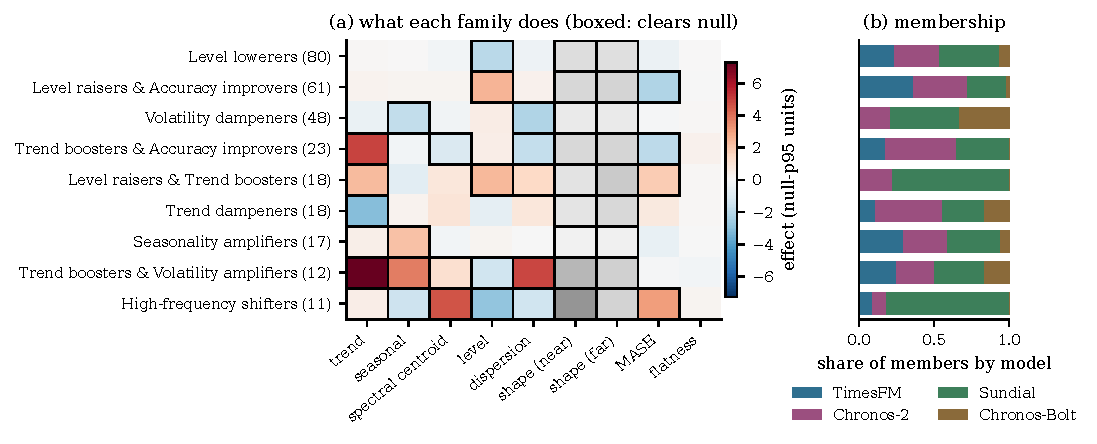
\includegraphics[width=\textwidth]{families.pdf}
\caption{The nine causal-effect families. (a) Family centroid in null units, signed as what the feature does
(red raises, blue lowers; boxed cells clear the null; shape distances unsigned, gray). (b) Membership by model. Source: \texttt{sae/concept\_families.json}.}
\label{fig:families}
\end{figure}
